%\documentclass[a4paper,superscriptaddress,11pt]{quantumarticle}
%\documentclass[aps,twocolumn,longbibliography,english,superscriptaddress]{revtex4-1}
\documentclass{article}
\usepackage[preprint]{neurips_2020}
%\documentclass[a4paper,superscriptaddress,11pt]{article}
\pdfoutput=1
\usepackage[colorlinks=true,urlcolor=blue,citecolor=blue,linkcolor=blue]{hyperref}
\usepackage[english]{babel}
\usepackage[utf8]{inputenc}
\usepackage[T1]{fontenc}
\usepackage{amssymb}
\usepackage{tabularx}
\usepackage{upquote}
\usepackage{subcaption}
\usepackage{multicol}
%\usepackage{caption}
%\usepackage[plain]{algorithm}
\usepackage[ruled, vlined]{algorithm2e}
\usepackage{algpseudocode}
\usepackage{rotating}
%\usepackage{cite}
\usepackage{booktabs}
%\usepackage{unicode-math}
%\usepackage{algorithm}% http://ctan.org/pkg/algorithm
%\usepackage{algpseudocode}% http://ctan.org/pkg/algpseudocode
\usepackage{xcolor}% http://ctan.org/pkg/xcolor
\makeatletter
\newsavebox{\@brx}
\newcommand{\llangle}[1][]{\savebox{\@brx}{\(\m@th{#1\langle}\)}%
  \mathopen{\copy\@brx\kern-0.5\wd\@brx\usebox{\@brx}}}
\newcommand{\rrangle}[1][]{\savebox{\@brx}{\(\m@th{#1\rangle}\)}%
  \mathclose{\copy\@brx\kern-0.5\wd\@brx\usebox{\@brx}}}
\makeatother
\usepackage{bbm}
\usepackage{jlcode}
\usepackage{graphicx}
\usepackage{amsmath,color,amsthm}
\usepackage{mathrsfs}
\usepackage{float}
\usepackage[normalem]{ulem}
\usepackage{indentfirst}
\usepackage{txfonts}
\usepackage[epsilon, tsrm, altpo]{backnaur}

\newcolumntype{b}{X}
\newcolumntype{s}{>{\hsize=.7\hsize}X}
\usepackage{listings}
\lstset{
    language=Julia,
    basicstyle=\ttfamily\scriptsize,
    numberstyle=\scriptsize,
    % numbers=left,
    backgroundcolor=\color{gray!7},
    %backgroundcolor=\color{white},
    %frame=single,
    xleftmargin=2em,
    tabsize=2,
    rulecolor=\color{black!15},
    %title=\lstname,
    %escapeinside={\%(*}{*)},
    breaklines=true,
    %breakatwhitespace=true,
    %framextopmargin=2pt,
    %framexbottommargin=2pt,
    frame=bt,
    extendedchars=true,
    inputencoding=utf8,
    columns=fullflexible,
}

\tolerance=1
\emergencystretch=\maxdimen
\hyphenpenalty=1000
\hbadness=1000

\makeatletter

%%%%%%%%%%%%%%%%%%%%%%%%%%%%%% User specified LaTeX commands.

%Journal reference.  Comma sets off: name, vol, page, year
\def\journal #1, #2, #3, 1#4#5#6{{\sl #1~}{\bf #2}, #3 (1#4#5#6) }
\def\pr{\journal Phys. Rev., }
\def\prb{\journal Phys. Rev. B, }
\def\prl{\journal Phys. Rev. Lett., }
\def\pl{\journal Phys. Lett., }
%\def\np{\journal Nucl. Phys., }


%%%%%%%%%%%%%%%%%%%%%%%%%%%%%%%%%%%%%%%%%%%%%%%%%%%%%%%%%%%%%%%%%%%%%%%%%%%%%%%%%%%%%%%%%%%%%%%%%%%%%%%%%%%%%%%%%%%%%%%%%%%%%%%%%%%%%%%%%%%%%%%%%%%%%%%%%%%%%%%%%%%%%%%%%%%%%%%%%%%%%%%%%%%%%%%%%%%%%%%%%%%%%%%%%%%%%%%%%%%%%%%%%%%%%%%%%%%%%%%%%%%%%%%%%%%%


%\usepackage{CJK}
%\usepackage[colorlinks, citecolor=blue]{hyperref}
\DeclareMathOperator*{\argmax}{arg\,max}

%%%%%% Shortcut related
\newcommand{\<}{\langle}
\renewcommand{\>}{\rangle}
\newcommand{\out}{{\vx^L}}
\newcommand{\inp}{{\vx^0}}
\newcommand{\cquad}{{{ }_{\quad}}}
\newcommand{\pluseq}{\mathrel{+}=}
\newcommand{\minuseq}{\mathrel{-}=}
\newcommand{\vx}{{\mathbf{x}}}
\newcommand{\vg}{{\mathbf{g}}}
\newcommand{\vp}{{\mathbf{p}}}
\newcommand{\vy}{{\mathbf{y}}}
\newcommand{\Var}{{\mathrm{Var}}}
\newcommand{\Mean}{{\mathrm{E}}}
\newcommand{\vvalue}{{\texttt{value}}}
\newcommand{\grad}{{\texttt{grad}}}
\newcommand{\parameter}{{\texttt{parameter}}}
%%%%%% Convention related
\newcommand{\SWAP}{{\rm SWAP}}
\newcommand{\CNOT}{{\rm CNOT}}
\newcommand{\X}{{\rm X}}
\renewcommand{\H}{{\rm H}}
\newcommand{\Rx}{{\rm Rx}}
\renewcommand{\v}[1]{{\bf #1}}
\newcommand{\dataset}{{\mathcal{D}}}
\newcommand{\wfunc}{{\psi}}
\newcommand{\SU}{{\rm SU}}
\newcommand{\UU}{{\rm U}}
\newcommand{\thetav}{{\boldsymbol{\theta}}}
\newcommand{\gammav}{{\boldsymbol{\gamma}}}
\newcommand{\thetai}{{\theta^\alpha_l}}
\newcommand{\Expect}{{\mathbb{E}}}
\newcommand{\Tr}{{\rm Tr}}
\newcommand{\etc}{{\it etc~}}
\newcommand{\etal}{{\it etal~}}
\newcommand{\xset}{\mathbf{X}}
\newcommand{\fl}{\texttt{fl}}
\newcommand{\pdata}{\mathbf{\pi}}
\newcommand{\q}{\mathbf{q}}
\newcommand{\epdata}{\mathbf{\hat{\pi}}}
\newcommand{\gammaset}{\boldsymbol{\Gamma}}
\newcommand{\ei}{{\mathbf{e}_l^\alpha}}
\newcommand{\vtheta}{{\boldsymbol{\theta}}}
\newcommand{\sigmag}{{\nu}}
\newcommand{\sigmai}[2]{{\sigma^{#2}_{#1}}}
\newcommand{\qi}[1]{{q^{\alpha_{#1}}_{#1}}}
\newcommand{\BAS}{Bars-and-Stripes}
\newcommand{\circled}[1]{\raisebox{.5pt}{\textcircled{\raisebox{-.9pt} {#1}}}}

\newcommand{\qexpect}[1]{{\left\langle #1\right\rangle}}
\newcommand{\expect}[2]{{\mathop{\mathbb{E}}\limits_{\substack{#2}}\left[#1\right]}}
\newcommand{\var}[2]{{\mathop{\mathrm{Var}}\limits_{\substack{#2}}\left(#1\right)}}
\newcommand{\pshift}[1]{{p_{\thetav+#1}}}
\newcommand{\upcite}[1]{\textsuperscript{\cite{#1}}}
\newcommand{\Eq}[1]{Eq.~(\ref{#1})}
\newcommand{\Fig}[1]{Fig.~\ref{#1}}
\newcommand{\Lst}[1]{Listing.~\ref{#1}}
\newcommand{\Ref}[1]{Ref.~\cite{#1}}
\newcommand{\Tbl}[1]{Table~\ref{#1}}
\newcommand{\Sec}[1]{Sec.~\ref{#1}}
\newcommand{\bra}[1]{\mbox{$\left\langle #1 \right|$}}
\newcommand{\ket}[1]{\mbox{$\left| #1 \right\rangle$}}
\newcommand{\braket}[2]{\mbox{$\left\langle #1 | #2 \right\rangle$}}
\newcommand{\tr}[1]{\mathrm{tr}\mbox{$\left[ #1\right]$}}

\newcommand{\ra}[1]{\renewcommand{\arraystretch}{#1}}

%%%%%% Comment related
\newcommand{\red}[1]{[{\bf  \color{red}{LW: #1}}]}
\newcommand{\xred}[1]{[{\bf  \color{red}{\sout{LW: #1}}}]}
\newcommand{\blue}[1]{[{\bf  \color{blue}{JG: #1}}]}
\newcommand{\violet}[1]{[{\bf  \color{violet}{MLS: #1}}]}
\newcommand{\green}[1]{[{\bf  \color{green}{TZ: #1}}]}
\newcommand{\xgreen}[1]{[{\bf  \color{green}{\sout{TZ: #1}}}]}
\newcommand{\xblue}[1]{[{\bf  \color{blue}{\sout{JG: #1}}}]}
\newcommand{\material}[1]{\iffalse[{\bf  \color{cyan}{Material: #1}}]\fi}
\newcommand{\orange}[1]{\iffalse[{\bf  \color{orange}{Jo: #1}}]\fi}

\newtheorem{theorem}{\textit{Theorem}}
\theoremstyle{definition}\newtheorem{definition}{\textit{Definition}}

\makeatother

\begin{document}
\title{Differentiate Everything with a Reversible Domain-Specific Language}

\author{Jin-Guo Liu\\
Institute of Physics, Chinese Academy of Sciences,\\Beijing 100190, China\\
\texttt{cacate0129@iphy.ac.cn}\\
\And
Taine Zhao\\
Department of Computer Science, University of Tsukuba\\
\texttt{thaut@logic.cs.tsukuba.ac.jp}\\
}
%\author{Lei Wang}
%\email{wanglei@iphy.ac.cn}
%\affiliation{Institute of Physics, Chinese Academy of Sciences, Beijing 100190, China}
%\affiliation{CAS Center for Excellence in Topological Quantum Computation, University of Chinese Academy of Sciences, Beijing 100190, China}
%\affiliation{Songshan Lake Materials Laboratory, Dongguan, Guangdong 523808, China}

%\author{Jin-Guo Liu}
%\email{cacate0129@iphy.ac.cn}
%\affiliation{Institute of Physics, Chinese Academy of Sciences, Beijing 100190, China}

%\author{Taine Zhao}
%\affiliation{Department of Computer Science, University of Tsukuba}

\maketitle

\begin{abstract}
    Traditional machine instruction level reverse mode automatic differentiation (AD) suffers from the problem of having a space overhead that linear to time in order to trace back the computational state, which is also the source of bad time performance. In reversible programming, a program can be executed bi-directionally, which means we do not need extra design to trace back the computational state. This paper answers the question that how practical it is to implement a machine instruction level reverse mode AD in a reversible programming language. By implementing sparse matrix operations and some machine learning applications in our reversible eDSL NiLang, and benchmark the performance with state-of-the-art AD frameworks, our answer is a clear positive.
    NiLang is an open source r-Turing complete reversible eDSL in Julia. It empowers users the flexibility to tradeoff time, space, and energy rather than caching data into a global tape. Manageable memory allocation makes it a good tool to differentiate GPU kernels too.
\end{abstract}

%\begin{multicols}{2}
\section{Introduction}\label{sec:intro}
    Computing the gradients of a numeric model $f : \mathbb{R}^m \rightarrow \mathbb{R}^n$ plays a crucial role in scientific computing. Consider a computing process
\begin{align*}
    &\vx^1 = f_1(\vx^0)\\
    &\vx^2 = f_2(\vx^1)\\
    &\ldots\\
    &\vx^L = f_L(\vx^{L-1})
\end{align*}
where $x^0\in R^m$, $x^L\in R^n$, $L$ is the depth of computing.
The Jacobian of this program is a $n\times m$ matrix $J_{ij} \equiv \frac{\partial x^L_i}{\partial x_j^0}$, where $x_j^0$ and $x_i^L$ are single elements from inputs and outputs.
Computing the Jacobian or part of the Jacobian automatically is what we called automatic differentiation (AD). It can be classified into three classes, the forward mode AD, the backward mode AD and the mixed mode AD~\cite{Hascoet2013}.
    The forward mode AD computes the Jacobian matrix elements related to a single input using the chain rule $\frac{\partial \vx^k}{\partial x^0_j} = \frac{\partial \vx^k}{\partial \vx^{k-1}}\frac{\partial \vx^{k-1}}{\partial x^0_j}$ with $j$ the column index, while a backward mode AD computes Jacobian matrix elements related to a single output using the chain rule in the reverse direction $\frac{\partial \vx^L_i}{\partial x^{k-1}} = \frac{\partial \vx^L_i}{\partial \vx^{k}}\frac{\partial \vx^{k}}{\partial x^{k-1}}$ with $i$ the row index.
    In variational applications where the loss function always outputs a scalar, the backward mode AD is preferred.
However, implementing backward mode AD is harder than implementing its forward mode counterpart, because it requires propagating the gradients in the inverse direction of computing the loss. The backpropagation of gradients requires
\begin{enumerate}
    \item an approach to trace back the computational process,
    \item caching variables required for computing gradients.
\end{enumerate}
    %The computational process is often represented as a computational graph, a directed acyclic graph (DAG) representing the relationship between data and functions. Comparing with a general computer program, a computational graph does not have mutable variables and control flows.
    Most popular AD packages in the market implements the computational graph to solve above issues at the tensor level.
    In Pytorch~\cite{Paszke2017} and Flux~\cite{Innes2018a}, every variable has a tracker field. When applying a predefined primitive function on a variable, the variable's tracker field keeps track of this function as well as data needed in backpropagation.
    TensorFlow~\cite{Tensorflow2015} also implements the computational graph, but it builds a static computational graph as a description of the program before actual computation happens.
    %These packages all prefer tensor types, where the overhead of memory allocations is less significant.
    These frameworks sometimes fail to meet the diverse needs in research, for example, in physics research,
    \begin{enumerate}
        \item People need to differentiate over sparse matrix operations that are important for Hamiltonian engineering~\cite{Xie2020}, like solving dominant eigenvalues and eigenvectors~\cite{Golub2012},
        \item People need to backpropagate singular value decomposition (SVD) function and QR decomposition in tensor network algorithms to study the phase transition problem~\cite{Golub2012,Liao2019,Seeger2017,Wan2019,Hubig2019,Wan2019},
        \item People need to differentiate over a quantum simulation where each quantum gate is an inplace function that changes the quantum register directly~\cite{Luo2019}.
    \end{enumerate}
    %Scientists have put lots of effort to derive new backward rules for these needs.

    To solve these issues better, we need a hardware instruction level AD. Source code transformation based AD packages like Tapenade~\cite{Hascoet2013} and Zygote~\cite{Innes2018, Innes2019} are closer to this goal. They read the source code from a user and generate a new code that computes the gradients for users. However, these packages have their own limitations too. In many practical applications, an elementary level differentiable program that might do billions of computations will cache intermediate results to a global storage. Frequent caching of data slows down the program significantly, and the memory usage will become a bottleneck as well. With these AD tools, it is still nearly impossible to automatically generate the backward rules for BLAS functions and sparse matrix operations with a performance comparable to the state-of-the-art.% A better solution to memory management must be found to make source-to-source AD practical.

    We propose to implement hardware instruction level AD on a reversible (domain-specific) programming language~\cite{Perumalla2013,Frank2017}. So that the intermediate states of a program can be traced backward with no extra effort. The overhead of reverse mode AD becomes the overhead of reversing a program, where the later has the advantage of efficient and controllable memory management. There have been many prototypes of reversible languages like Janus~\cite{Lutz1986}, R (not the popular one)~\cite{Frank1997}, Erlang~\cite{Lanese2018} and object-oriented ROOPL~\cite{Haulund2017}. % These languages have reversible control flow that allows users to input an additional postcondition in control flows to help programs run backward.
    In the past, the primary motivation of studying reversible programming is to support reversible computing devices~\cite{Frank1999} like adiabatic complementary metal–oxide–semiconductor (CMOS)~\cite{Koller1992}, molecular mechanical computing system~\cite{Merkle2018} and superconducting system~\cite{Likharev1977,Semenov2003}, where a reversible computing device is more energy-efficient from the perspective of information and entropy, or by the Landauer's principle~\cite{Landauer1961}.
    After decades of efforts, reversible computing devices are very close to providing productivity now. As an example, adiabatic CMOS can be a better choice in a spacecraft~\cite{Hanninen2014, Debenedictis2017}, where energy is more valuable than device itself.
    Reversible programming is interesting to software engineers too, because it is a powerful tool to schedule asynchronious events~\cite{Jefferson1985} and debug a program bidirectionally~\cite{Boothe2000}.
    However, the field of reversible computing faces the issue of having not enough funding in recent decade~\cite{Frank2017}. As a result, not many people studying AD know the marvelous designs in reversible computing. People have not connected it with automatic differentiation seriously, even though they have many similarities. This paper aims to break the information barrier between the machine learning community and the reversible programming community in our work and provide yet another strong motivation to develop reversible programming.

    In this paper, we first introduce the language design of a reversible programming language and introduce our reversible eDSL NiLang in \Sec{sec:lang}.
    In \Sec{sec:bp}, we explain the implementation of automatic differentiation in this eDSL.
    In \Sec{sec:benchmark}, we benchmark the performance of NiLang with other AD packages and explain why reversible programming AD is fast.
    In the appendix, we show the detailed language design of NiLang, show some examples used in the benchmark, discuss several important issues including the time-space  tradeoff, reversible instructions and hardware, and finally, an outlook to some open problems to be solved.


\section{Language design}\label{sec:lang}

    \subsection{Introductions to reversible language design}
    In a modern programming language, functions are pushed to a global stack for scheduling. The memory layout of a function consists of input arguments, a function frame with information like the return address and saved memory segments, local variables, and working stack. After the call, the function clears run-time information, only stores the return value. In reversible programming, this kind of design is no longer the best practice. One can not discard input variables and local variables easily after a function call, since discarding information may ruin reversibility. For this reason, reversible functions are very different from irreversible ones from multiple perspectives.

\subsubsection{Memory management}
    A distinct feature of reversible memory management is, the content of a variable must be known when it is deallocated.
    We denote the allocation of a zero emptied memory as \texttt{x $\leftarrow$ 0}, and the corresponding deallocation as \texttt{x $\rightarrow$ 0}.
    A variable $x$ can be allocated and deallocated in a local scope, which is called an ancilla.
    It can also be pushed to a stack and used later with a pop statement.
    This stack is similar to a traditional stack, except it zero-clears the variable after pushing and presupposes that the variable being zero-cleared before popping.
Knowing the contents in the memory when deallocating is not easy. Hence Charles H. Bennett introduced the famous compute-copy-uncompute paradigm~\cite{Bennett1973} for reversible programming.

\subsubsection{Control flows}
One can define reversible \texttt{if}, \texttt{for} and \texttt{while} statements in a slightly different way comparing with its irreversible counterpart. The reversible \texttt{if} statement is shown in \Fig{fig:controlflow} (a). Its condition statement contains two parts, a precondition and a postcondition. The precondition decides which branch to enter in the forward execution, while the postcondition decides which branch to enter in the backward execution. After executing the specific branch, the program checks the consistency between precondition and postcondition to make sure they are consistent.
The reversible \texttt{while} statement in \Fig{fig:controlflow} (b) also has two condition fields. Before executing the condition expressions, the program preassumes the postcondition is false.
After each iteration, the program asserts the postcondition to be true. In the reverse pass, we exchange the precondition and postcondition.
The reversible \texttt{for} statement is similar to irreversible ones except that after executing the loop, the program checks the values of these variables to make sure they are not changed. In the reverse pass, we exchange \texttt{start} and \texttt{stop} and inverse the sign of \texttt{step}.
\begin{figure}
    \centerline{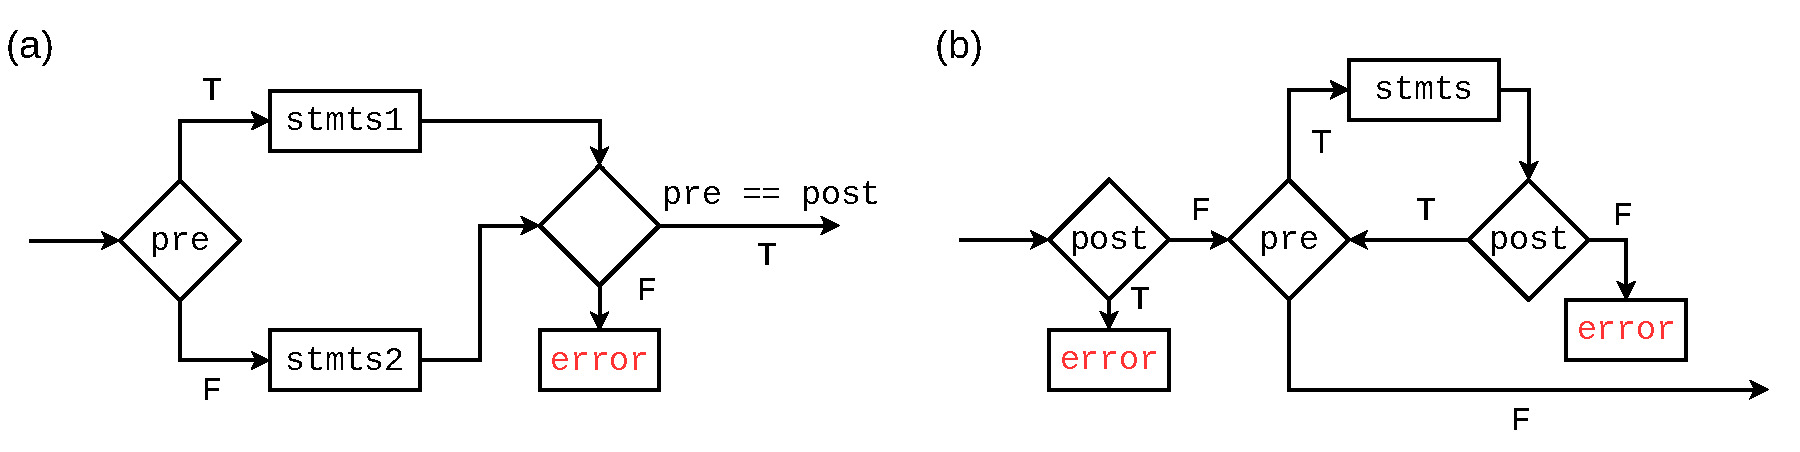
\includegraphics[width=0.9\columnwidth,trim={0 0cm 0 0cm},clip]{controlflow_v2.pdf}}
    \caption{The flow chart for reversible (a) \texttt{if} statement and (b) \texttt{while} statement. ``pre'' and ``post'' represents precondition and postconditions respectively.}\label{fig:controlflow}
\end{figure}

\subsubsection{Arithmetic instructions}
Every arithmetic instruction has a unique inverse that can undo the changes.
\begin{itemize}
    \item For logical operations, \texttt{y $\veebar$= f(args...)} is self reversible.
    \item For integer and floating point arithmetic operations, we treat \texttt{y += f(args...)} and \texttt{y -= f(args...)} as reversible to each other. Here \texttt{f} can be an arbitrary pure function such as \texttt{identity}, \texttt{*}, \texttt{/} and \texttt{\^}. Let's forget the floating point rounding errors for the moment and discuss in detail in the supplimentary materials.
    \item For logartihmic number and tropical number algebra~\cite{Speyer2009}, \texttt{y *= f(args...)} and \texttt{y /= f(args...)} as reversible to each other. Notice the zero element ($-\infty$) in the Tropical algebra is not considered here.
\end{itemize}
Besides the above two types of operations, \texttt{SWAP} operation that exchanges the contents in two memory spaces is also widely used in reversible computing systems.

\subsection{Differetiable Reversible eDSL: NiLang}
    We develop an embedded domain-specific language (eDSL) NiLang in Julia language~\cite{Bezanson2012,Bezanson2017} that implements reversible programming. One can write reversible control flows, instructions, and memory managements inside this macro.
Julia is a popular language for scientific programming. We choose Julia as the host language for multiple purposes. The most important consideration is speed that crucial for a machine instruction level AD. Its clever design of type inference and just in time compiling provides a C like speed.
Also, it has a rich ecosystem for meta-programming. The package for pattern matching \href{https://github.com/thautwarm/MLStyle.jl}{MLStyle} allow us to define an eDSL conveniently. Last but not least, its multiple-dispatch provides the polymorphism that will be used in our AD engine.
%In the past, we see many implementations of AD languages work as an independent language.
%However, we hope our eDSL can benefit people in Julia's community directly.
The main feature of NiLang is contained in a single macro \texttt{@i} that compiles a reversible function.
We can use \texttt{macroexpand} to show the compiling a reversible function to the native Julia function.

\begin{minipage}{.88\columnwidth}
\begin{lstlisting}
julia> using NiLangCore, MacroTools

julia> MacroTools.prettify(@macroexpand @i function f(x, y)
           SWAP(x, y)
       end)
quote
    $(Expr(:meta, :doc))
    function $(Expr(:where, :(f(x, y))))
        dove = wrap_tuple(SWAP(x, y))
        x = dove[1]
        y = dove[2]
        (x, y)
    end
    if NiLangCore._typeof(f) != _typeof(~f)
        function $(Expr(:where, :((hummingbird::_typeof(~f))(x, y))))
            toad = wrap_tuple((~SWAP)(x, y))
            x = toad[1]
            y = toad[2]
            (x, y)
        end
    end
end
\end{lstlisting}
\end{minipage}

Here, the version of NiLang is v0.4.0.
Macro \texttt{@i} generates two functions that reversible to each other \texttt{f} and \texttt{$\sim$f}. \texttt{$\sim$f} is an callable of type \texttt{Inv\{typeof(f)\}}, where the type parameter \texttt{typeof(f)} stands for the type of the function \texttt{f}.
In the body of \texttt{f}, \texttt{NiLangCore.wrap\_tuple} is used to unify output data types to tuples.
The outputs of \texttt{SWAP} are assigned back to its input variables.
At the end of this function, this macro attaches a return statement that returns all input variables.

The compilation of a reversible function to native Julia functions is consisted of three stages: \textit{preprocessing}, \textit{reversing} and \textit{translation}.
\Fig{fig:compiling} shows the compilation of the complex valued log function body, which is originally defined as follows.

\begin{minipage}{.88\columnwidth}
\begin{lstlisting}[mathescape=true,caption={Reversible implementation of the complex valued log function.},label={lst:complex}]
@i function (:+=)(log)(y!::Complex{T}, x::Complex{T}) where T
    @routine begin
        n ← zero(T)
        n += abs(x)
    end
    y!.re += log(n)
    y!.im += angle(x)
    ~@routine
end
\end{lstlisting}
\end{minipage}

\begin{figure}
    \centerline{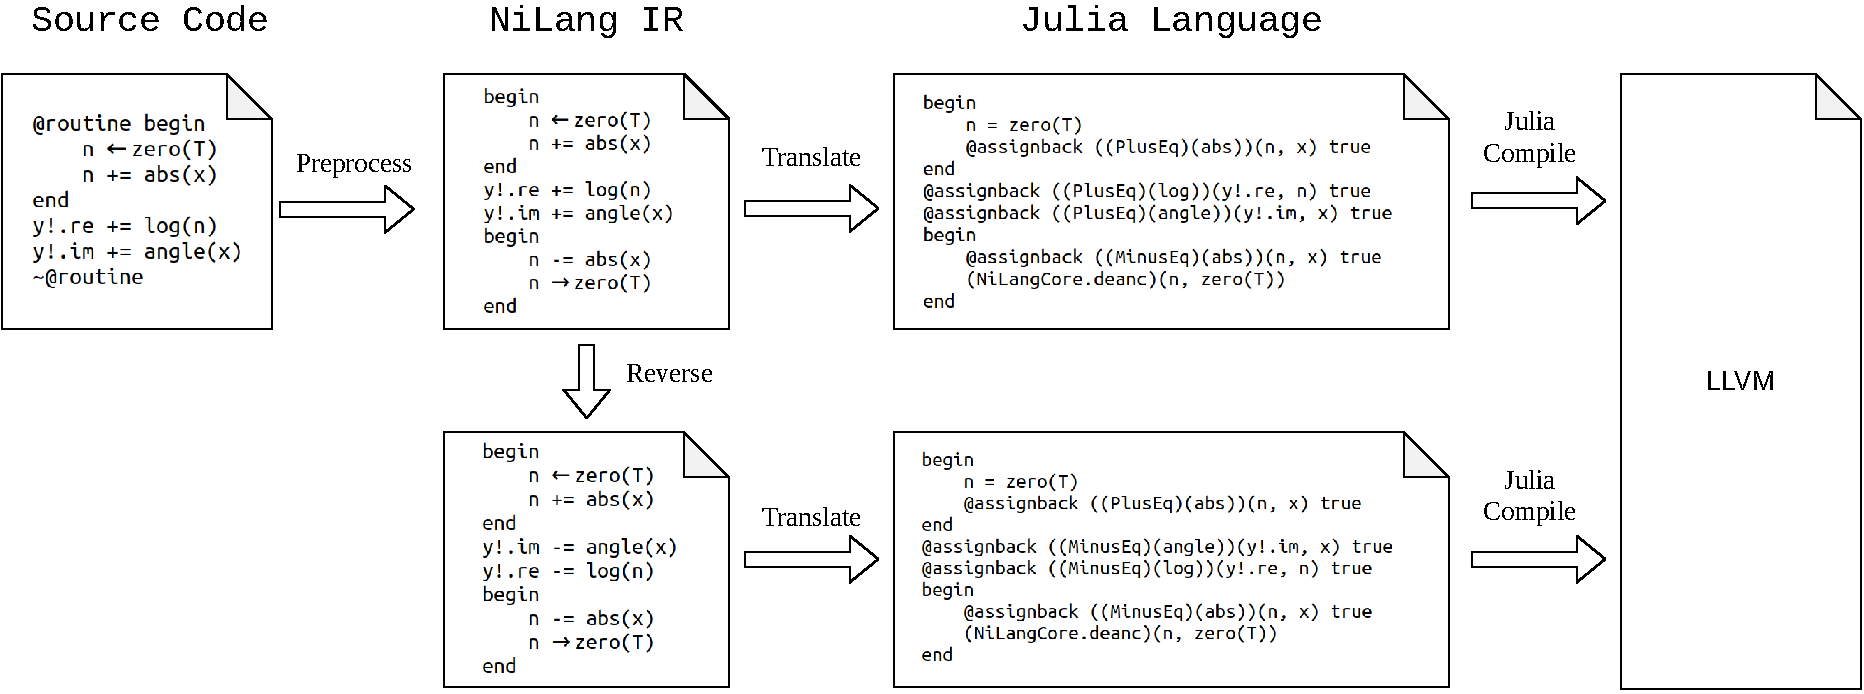
\includegraphics[width=0.95\columnwidth,trim={0cm 0cm 0cm 0cm},clip]{compiling_v2.pdf}}
    \caption{Compiling the body of the complex valued log function defined in \Lst{lst:complex}.}\label{fig:compiling}
\end{figure}

In the \textit{preprocessing} stage, the compiler pre-processes human inputs to reversible NiLang IR.
The preprocessor removes redundant grammars and expands shortcuts. In the left most code box in \Fig{fig:compiling}, one uses \texttt{@routine <stmt>} statement to record a statement, and \texttt{$\sim$@routine} to insert the corresponding inverse statement for uncomputing.
The computing-uncomputing macros \texttt{@routine} and \texttt{$\sim$@routine} is expanded in this stage.
Here, one can input ``$\leftarrow$'' and ``$\rightarrow$'' by typing ``$\backslash$leftarrow[TAB KEY]'' and ``$\backslash$rightarrow[TAB KEY]'' respectively in a Julia editor or REPL.
In the \textit{reversing} stage, based on this symmetric and reversible IR, the compiler generates reversed statements.
In the \textit{translation} stage, the compiler translates this reversible IR as well as its inverse to native Julia code. It adds \texttt{@assignback} before each function call, inserts codes for reversibility check, and handle control flows.
We can expand the \texttt{@assignback} macro to see the compiled expression.
As a final step, the compiler attaches a return statement that returns all updated input arguments at the end of a function definition.
Now, the function is ready to execute on the host language.

\section{Reversible automatic differentiation}\label{sec:bp}

\subsection{First order gradient}\label{sec:jacobian}
\begin{figure}
    \centerline{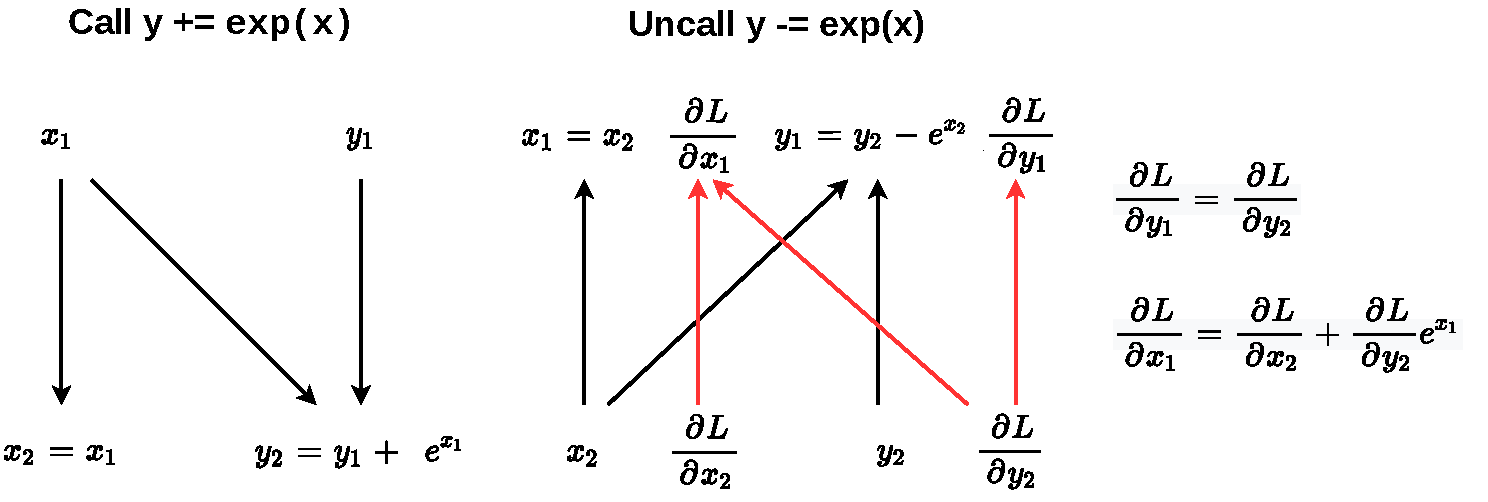
\includegraphics[width=0.8\columnwidth,trim={0 0cm 0 0cm},clip]{reversead.pdf}}
    \caption{Binding the adjoint rule of \texttt{y+=exp(x)} to its uncomputing program.}\label{fig:reversead}
\end{figure}

The computation of gradients in NiLang contains two parts, computing and uncomputing. In the computing stage, the program marches forward and computes outputs.
In the uncomputing stage, we attach each scalar and array element with an extra gradient field and feed them into the inverse function. To composite data type with a gradient field is called \texttt{GVar}. As shown in \Fig{fig:reversead}, when an instruction is uncalled, we first uncompute the value field of \texttt{GVar}s to $x_1$ and $y_1$, using the input information, we then update the gradient fields according to the formula in the right panel. The binding utilizes the multiple dispatch in Julia, where a function can be dynamically dispatched based on the run time type of more than one of its arguments. Here, we dispatch a inverse instruction with input type \texttt{GVar} to the \texttt{(:-=)(exp)} instruction.

\begin{minipage}{.88\columnwidth}
\begin{lstlisting}[mathescape=true]
@i @inline function (:-=)(exp)(out!::GVar, x::GVar{T}) where T
    @routine @invcheckoff begin
        anc1 ← zero(value(x))
        anc1 += exp(value(x))
    end
    value(out!) -= identity(anc1)
    grad(x) += grad(out!) * anc1
    ~@routine
end
\end{lstlisting}
\end{minipage}

Here, the first four lines is the \texttt{@routine} statement that computes $e^{x_2}$ and store the value into an ancilla. The 5th line updates the \texttt{value} dataview of \texttt{out!}. The 6th line updates the gradient fields of \texttt{x} and \texttt{y} by applying the adjoint rule of \texttt{(:+=)(exp)}. Finally, \texttt{~@routine} uncomputes \texttt{anc1} so that it can be returned to the ``memory pool''.
One does not need to define the similar function on \texttt{(:+=)(exp)} because macro \texttt{@i} will generate it automatically. Notice that taking inverse and computing gradients commute~\cite{Mcinerney2015}.

\subsection{Hessians, complex numbers and CUDA kernels}
Combining the uncomputing program in NiLang with dual-numbers is a simple yet efficient way to obtain Hessians.
The dual number is the scalar type for computing gradients in the forward mode AD, it wraps the original scalar with a extra gradient field. The gradient field of a dual number is updated automatically as the computation marches forward.
By wrapping the elementary type with \texttt{Dual} defined in package ForwardDiff~\cite{Revels2016} and throwing it into the gradient program defined in NiLang,
one obtains one row/column of the Hessian matrix straightforward.
We will show a benchmark in \Sec{sec:graphbench}.

To differentiate complex numbers, we re-implemented complex instructions reversibly. For example, with the reversible function defined in in \Lst{lst:complex}, we can differentiated complex valued log with no extra effort.

CUDA programming is playing a significant role in high-performance computing. In Julia, one can write GPU compatible functions in native Julia language with \href{https://github.com/JuliaGPU/KernelAbstractions.jl}{KernelAbstractions}~\cite{Besard2018}.
Since NiLang does not push variables into stack automatically for users, it is safe to write differentiable GPU kernels with NiLang.
We will show this feature in the benchmarks of bundle adjustment (BA) in \Sec{sec:ba}.
Here, one should notice that the shared read in forward pass will become shared write in the backward pass, which may result in incorrect gradients. We will review this issue in the supplimentary material.

\section{Benchmarks}\label{sec:benchmark}

In the following benchmarks the CPU device is Intel(R) Xeon(R) Gold 6230 CPU @ 2.10GHz, and the GPU device is Nvidia Titan V.
% the GPU time is estimated by broadcasting the gradient function on CUDA array of size $2^{17}$ and taking the average.
For NiLang benchmarks, we have turned off the reversibility check off to achieve a better performance. Codes used in benchmarks could be found the in Examples section of supplimentary material.

\subsection{Sparse matrices}\label{sec:benchsparse}
We benchmarked the call, uncall and backward propagation time used for sparse matrix dot product and matrix multiplication.
Here, we estimate the time for back propagating gradients rather than including both forward and backward, since \texttt{mul!} does not output a scalar as loss.

\begin{table}[h!]\centering
\begin{minipage}{0.8\columnwidth}
\ra{1.3}
    \scalebox{1.0}{
        \begin{tabularx}{\textwidth}{bsb}\toprule
            \textbf{}     & \texttt{dot}         & \texttt{mul!} (complex valued) \\
            \hline
            Julia-O       & 3.493e-04   & 8.005e-05\\
            NiLang-O      & 4.675e-04   & 9.332e-05\\
            \hline
            NiLang-B      & 5.821e-04   & 2.214e-04\\
            \bottomrule
        \end{tabularx}
    }
    \caption{Absolute runtimes in seconds for computing the objectives (O) and the backward pass (B) of sparse matrix operations. The matrix size is $1000 \times 1000$, and the element density is $0.05$. The total time used in computing gradient can be estimated as a sum of ``O'' and ``B''.
    }\label{tbl:sparse}
\end{minipage}
\end{table}

The time used for computing backward pass is approximately 1.5-3 times the Julia's native forward pass.
This is because the instruction length of differentiating basic arithmetic instructions is longer than pure computing by a factor of 2 or more.


\subsection{Graph embedding problem}\label{sec:graphbench}
Since one can combine ForwardDiff and NiLang to obtain Hessians,
it is interesting to see how much performance we can get in differentiating the graph embedding program. The problem definition could be found in the supplimentary material.

\begin{table}[h!]\centering
    \small
\begin{minipage}{\columnwidth}
\ra{1.3}
    \scalebox{1.0}{
        \begin{tabularx}{\textwidth}{bssssssssss}\toprule
            $k$                      & 2          & 4          & 6          & 8          & 10         \\
            \hline
            Julia-O                  & 4.477e-06  & 4.729e-06  & 4.959e-06  & 5.196e-06  & 5.567e-06  \\
            NiLang-O                 & 7.173e-06  & 7.783e-06  & 8.558e-06  & 9.212e-06  & 1.002e-05  \\
            NiLang-U                 & 7.453e-06  & 7.839e-06  & 8.464e-06  & 9.298e-06  & 1.054e-05  \\
            \hline
            NiLang-G                 & 1.509e-05  & 1.690e-05  & 1.872e-05  & 2.076e-05  & 2.266e-05  \\
            ReverseDiff-G            & 2.823e-05  & 4.582e-05  & 6.045e-05  & 7.651e-05  & 9.666e-05  \\
            ForwardDiff-G            & 1.518e-05  & 4.053e-05  & 6.732e-05  & 1.184e-04  & 1.701e-04  \\
            Zygote-G                 & 5.315e-04  & 5.570e-04  & 5.811e-04  & 6.096e-04  & 6.396e-04  \\
            \hline
            (NiLang+F)-H             & 4.528e-04  & 1.025e-03  & 1.740e-03  & 2.577e-03  & 3.558e-03  \\
            ForwardDiff-H            & 2.378e-04  & 2.380e-03  & 6.903e-03  & 1.967e-02  & 3.978e-02  \\
            (ReverseDiff+F)-H        & 1.966e-03  & 6.058e-03  & 1.225e-02  & 2.035e-02  & 3.140e-02  \\
            \bottomrule
        \end{tabularx}
    }
    \caption{Absolute times in seconds for computing the objectives (O), uncall objective (U), gradients (G) and Hessians (H) of the graph embedding program.
    $k$ is the embedding dimension, the number of parameters is $10k$.
    }\label{tbl:graphembedding}
\end{minipage}
\end{table}

In \Tbl{tbl:graphembedding}, we show the the performance of different implementations by varying the dimension $k$. The number of parameters is $10k$.
As the baseline, (a) shows the time for computing the function call. We have reversible and irreversible implementations, where the reversible program is slower than the irreversible native Julia program by a factor of $\sim2$ due to the uncomputing overhead.
The reversible program shows the advantage of obtaining gradients when the dimension $k \geq 3$. The larger the number of inputs, the more advantage it shows due to the overhead proportional to input size in forward mode AD.
The same reason applies to computing Hessians, where the combo of NiLang and ForwardDiff gives the best performance for $k \geq 3$.

\subsection{Gaussian mixture model and bundle adjustment}\label{sec:ba}

We reproduced the benchmarks for Gaussian mixture model (GMM) and bundle adjustment (BA) in ~\Ref{Srajer2018} by re-writing the programs in a reversible style. We show the results in \Tbl{tbl:gmm} and \Tbl{tbl:ba}. In our new benchmarks, we also rewrite the ForwardDiff program for a fair benchmark, this explains the difference between our results and the original benchmark. The Tapenade data is obtained by executing the docker file provided by the original benchmark, which provides a baseline for comparison.

\begin{table}[h!]\centering
    \scriptsize
\begin{minipage}{\columnwidth}
\ra{1.3}
    \scalebox{1.0}{
        \begin{tabularx}{\textwidth}{bssssssss}\toprule
            \textbf{\# parameters} & 3.00e+1 & 3.30e+2 & 1.20e+3 & 3.30e+3 & 1.07e+4 & 2.15e+4 & 5.36e+4 & 4.29e+5\\
            \hline
            Julia-O       & 9.844e-03 & 1.166e-02 & 2.797e-01 & 9.745e-02 & 3.903e-02 & 7.476e-02 & 2.284e-01 & 3.593e+00  \\
            NiLang-O      & 3.655e-03 & 1.425e-02 & 1.040e-01 & 1.389e-01 & 7.388e-02 & 1.491e-01 & 4.176e-01 & 5.462e+00  \\
            Tapende-O     & 1.484e-03 & 3.747e-03 & 4.836e-02 & 3.578e-02 & 5.314e-02 & 1.069e-01 & 2.583e-01 & 2.200e+00\\
            \hline
            ForwardDiff-G & 3.551e-02 & 1.673e+00 & 4.811e+01 & 1.599e+02 & -         & -         & -         & -  \\
            NiLang-G      & 9.102e-03 & 3.709e-02 & 2.830e-01 & 3.556e-01 & 6.652e-01 & 1.449e+00 & 3.590e+00 & 3.342e+01  \\
            Tapenade-G    & 5.484e-03 & 1.434e-02 & 2.205e-01 & 1.497e-01 & 4.396e-01 & 9.588e-01 & 2.586e+00 & 2.442e+01\\
            \bottomrule
        \end{tabularx}
    }
    \caption{Absolute runtimes in seconds for computing the objective (O) and gradients (G) of GMM with 10k data points. ``-'' represents missing data due to not finishing the computing in limited time.}\label{tbl:gmm}
\end{minipage}
\end{table}

In the GMM benchmark, NiLang's objective function has overhead comparing with irreversible programs in most cases.
Except the uncomputing overhead, it is also because our naive reversible matrix-vector multiplication is much slower than the highly optimized BLAS function, where the matrix-vector multiplication is the bottleneck of the computation.
The forward mode AD suffers from too large input dimension in the large number of parameters regime.
Although ForwardDiff batches the gradient fields, the overhead proportional to input size still dominates.
The source to source AD framework Tapenade is faster than NiLang in all scales of input parameters,
but the ratio between computing the gradients and the objective function are close.
%The memory consumption of our reversible implementation is quite low.
%The peak memory is only slightly more than twice of the original program,
%where the factor 2 comes from wrapping each variable with an extra gradient field.

\begin{table}[h!]\centering
    \scriptsize
\begin{minipage}{\columnwidth}
\ra{1.3}
    \scalebox{1.0}{
        \begin{tabularx}{\textwidth}{bsssssss}\toprule
            \textbf{\# measurements} & 3.18e+4 & 2.04e+5 & 2.87e+5 & 5.64e+5 & 1.09e+6 & 4.75e+6 & 9.13e+6\\
            \hline
            Julia-O        & 2.020e-03 & 1.292e-02 & 1.812e-02 & 3.563e-02 & 6.904e-02 & 3.447e-01 & 6.671e-01\\
            NiLang-O       & 2.708e-03 & 1.757e-02 & 2.438e-02 & 4.877e-02 & 9.536e-02 & 4.170e-01 & 8.020e-01\\
            Tapenade-O     & 1.632e-03 & 1.056e-02 & 1.540e-02 & 2.927e-02 & 5.687e-02 & 2.481e-01 & 4.780e-01\\
            \hline
            ForwardDiff-J  & 6.579e-02 & 5.342e-01 & 7.369e-01 & 1.469e+00 & 2.878e+00 & 1.294e+01 & 2.648e+01\\
            NiLang-J       & 1.651e-02 & 1.182e-01 & 1.668e-01 & 3.273e-01 & 6.375e-01 & 2.785e+00 & 5.535e+00\\
            NiLang-J (GPU) & 1.354e-04 & 4.329e-04 & 5.997e-04 & 1.735e-03 & 2.861e-03 & 1.021e-02 & 2.179e-02\\
            Tapenade-J     & 1.940e-02 & 1.255e-01 & 1.769e-01 & 3.489e-01 & 6.720e-01 & 2.935e+00 & 6.027e+00\\
            \bottomrule
        \end{tabularx}
    }
    \caption{Absolute runtimes in seconds for computing the objective (O) and Jacobians (J) in bundle adjustment.}\label{tbl:ba}
\end{minipage}
\end{table}

In the BA benchmark, reverse mode AD shows slight advantage over ForwardDiff.
The bottleneck of computing this large sparse Jacobian is computing the Jacobian of a elementary function with 15 input arguments and 2 output arguments, where input space is larger than the output space.
In this instance, our reversible implementation is even faster than the source code transformation based AD framework Tapenade.
With KernelAbstractions, we run our zero allocation reversible program on GPU, which provides a >200x speed up.
%Running codes on GPU (in Julia) requires not introducing any memory allocation at the kernel level.
%NiLang provides user the flexibility to manage the memory allocation instead of using a global stack.

\section{Acknowledgments}
Jin-Guo Liu thank Lei Wang for motivating the project with possible applications to reversible integrator, normalizing flow, and neural ODE.
Johann-Tobias Schäg for deepening the discussion about reversible programming with his mathematicians head.
Marisa Kiresame and Xiu-Zhe Luo for discussion on the implementation details of source-to-source automatic differentiation,
Shuo-Hui Li for helpful discussion on differential geometry, Tong Liu and An-Qi Chen for helpful discussion on quantum adders and multipliers, Ying-Bo Ma for correcting typos by submitting pull requests, Chris Rackauckas for helpful discussion on reversible integrator, Mike Innes for reviewing the comments about Zygote, Jun Takahashi for discussion about the graph embedding problem, Simon Byrne and Chen Zhao for helpful discussion on floating-point and logarithmic numbers.
The authors are supported by the National Natural Science Foundation of China under Grant No.~11774398, the Strategic Priority Research Program of Chinese Academy of Sciences Grant No.~XDB28000000.

\bibliographystyle{apsrev4-1}
\bibliography{invc}


\end{document}
